%-----------------------------------------------------------------
%	BOOTSTRAP: SIMPLE REGRESSION
%	!TEX root = ./../main.tex
%-----------------------------------------------------------------
\subsection{Test statistics to compare the two populations}\label{sec:statistics-intro}
The marginal analysis of the data performed in \Cref{ssec:univariate} suggests that there are slight differences in the $PDI$ and lifetime marginal distributions for the populations associated to the different SST classes, and thus their joint distribution.

However, theory suggests that there is no difference in the evolution of a tropical-cyclone once it is activated. Therefore, we should expect that
\begin{align}
	f(Y \mid X = x)_{\text{low}} = f(Y \mid X = x)_{\text{high}}
	\tag{\ref{eq:hypothesis} bis}
	.
\end{align}

To analyse this, we propose following null hypothesis:
\begin{align}
	H_{0} : \hat{\beta}_{0,h} = \hat{\beta}_{0,l} \wedge \hat{\beta}_{1,h} = \hat{\beta}_{1,l}
	.
\end{align}

The simplest way to test this is to build and calculate statistics that compare both populations that are near to zero if $H_{0}$ is true. There are many possible test statistics that could help us test the null hypothesis, but assuming both populations follow the same trend under a linear regression approach, it seems straightforward to compare the coefficient estimates directly:
\begin{align}
	T^{(1)} = \abs{\hat{\beta}_{0,h} - \hat{\beta}_{0,l}}
	\qc
	T^{(2)} = \abs{\hat{\beta}_{1,h} - \hat{\beta}_{1,l}}
	\qc
	T^{(3)} = \abs{ R^{2}_{h} - R^{2}_{l} } \label{eq:h0-stat-simple} .
\end{align}

\textcite{Polko-Zajac2016} propose alternative statistics that not only consider the nominal value of the coefficient estimates, but take into account their standard errors as well:
\begin{align}
	T^{(4)} = \frac{\abs{\hat{\beta}_{0,h} - \hat{\beta}_{0,l}}}{\se{\hat{\beta}_{0,h} - \hat{\beta}_{0,l}}}
	\qc
	T^{(5)} = \frac{\abs{\hat{\beta}_{1,h} - \hat{\beta}_{1,l}}}{\se{\hat{\beta}_{1,h} - \hat{\beta}_{1,l}}}
	\qc
	T^{(6)} = T^{(4)} + T^{(5)} \label{eq:h0-stat-polko} .
\end{align}

%-----------------------------------------------------------------
\subsection{Analysis using ordinary least squares}\label{sec:reg-analysis-data}

Before we can calculate the test statistics $T^{(i)}$, we need to fit a linear regression model on the data using the OLS method.

In \Cref{fig:natl-scatterplot} we can see the regression models that fit the joint bivariate lognormal distribution of $PDI$ and lifetime of storms of the populations associated to the different SST classes for the North Atlantic basin. The coefficient estimates obtained for each of the four resulting regression models are shown in \Cref{tab:natl-ols-coefs}.

With the obtained coefficient estimates we calculate the test statistics $T^{(i)}$associated to the model $PDI(\text{lifetime})$ and the inverse $\text{lifetime}(PDI)$ to compare occurrences in low-SST years and in high-SST years for the North Atlantic basin. These are shown in \Cref{tab:base-natl-ols-statistics}.

\medskip
We can see that the regressions for low-SST years and high-SST years are statistically compatible (\Cref{tab:natl-ols-coefs}), although for the $PDI(\text{lifetime})$ regression the coefficients seem to be much closer, as can be clearly seen in \Cref{fig:natl-scatterplot}.

The results shown in \Cref{tab:base-natl-ols-statistics} might be surprising at first, especially the value of $T^{(1)}$ for the $\text{lifetime}(PDI)$ regression, as it is quite big. This is actually an expected result that derives from the relative position of the joint distributions for the two SST classes.

\begin{figure}[H]
	\centering
	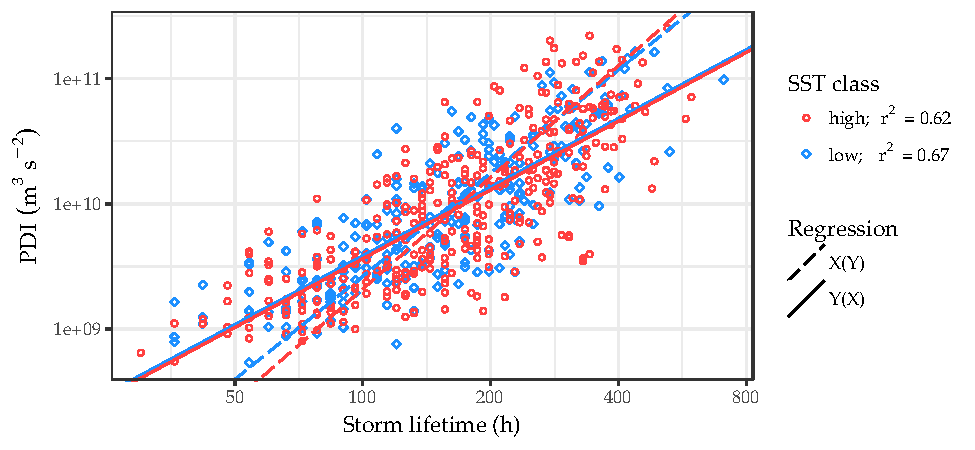
\includegraphics[width=\textwidth]{images/scatterplot-natl}
	\caption{Scatterplot of the joint distribution and regression analysis for the $PDI$ and lifetime of storms for the North Atlantic basin}
	\label{fig:natl-scatterplot}
\end{figure}

\begin{table}[H]
	\centering
	\begin{tabular}{cccccc}
		\toprule
		\toprule
		$X$ & $Y$ & SST class & $\hat{\beta}_{0}$ & $\hat{\beta}_{1}$ & $R^{2}$ \\
		\midrule
		\multirow{2}{*}{lifetime} & \multirow{2}{*}{$PDI$}
		 & Low  & \num{ 5.94 \pm 0.18} & \num{1.82 \pm 0.08} & \num{0.67} \\ % \pm 0.05} \\
		&& High & \num{ 5.91 \pm 0.17} & \num{1.83 \pm 0.08} & \num{0.62} \\ % \pm 0.04} \\
		\midrule
		\multirow{2}{*}{$PDI$} & \multirow{2}{*}{lifetime}
		 & Low  & \num{-1.44 \pm 0.16} & \num{0.37 \pm 0.02} & \num{0.67} \\ % \pm 0.05} \\
		&& High & \num{-1.14 \pm 0.14} & \num{0.34 \pm 0.01} & \num{0.62} \\ % \pm 0.04} \\
		\bottomrule
	\end{tabular}
	\caption{Linear regression coefficients obtained performing OLS on the North Atlantic basin data}
	\label{tab:natl-ols-coefs}
\end{table}

% The value of the studied statistics $T^{(i)}$ obtained from the N.~Atl. data set can be seen in \Cref{tab:base-natl-ols-statistics}.
\begin{table}[H]
	\centering
	\begin{tabular}{cccccccc}
	\toprule
	\toprule
	$X$   & $Y$   & $T^{(1)}$ & $T^{(2)}$ & $T^{(3)}$ & $T^{(4)}$ & $T^{(5)}$ & $T^{(6)}$ \\
	\midrule
	lifetime & $PDI$ & $0.025$ & $0.001$ & $0.051$ & $0.101$ & $0.010$ & $0.111$ \\
	$PDI$ & lifetime & $0.299$ & $0.028$ & $0.051$ & $1.388$ & $1.295$ & $2.683$ \\
	\bottomrule
	\end{tabular}
	\caption{Value of the test statistics for North Atlantic basin data set using OLS}
	\label{tab:base-natl-ols-statistics}
\end{table}

\bigskip
For the Northeast Pacific we have a similar situation. In \Cref{fig:epac-scatterplot} we can see the regression models that fit the joint bivariate lognormal distributions; the coefficient estimates obtained for each of these four resulting regression models are shown in \Cref{tab:epac-ols-coefs}. The values of the test statistics for this basin are shown in \Cref{tab:base-epac-ols-statistics}.


\medskip
We can see that the regressions for low-SST years and high-SST years are statistically compatible as well (\Cref{tab:epac-ols-coefs}). As it also happens for the North Atlantic, for the $PDI(\text{lifetime})$ regression the coefficients seem to be much closer, as can be clearly seen in \Cref{fig:epac-scatterplot}.

The results shown in \Cref{tab:base-epac-ols-statistics} are definitely surprising, in particular the value of $T^{(1)}$ for the $PDI(\text{lifetime}$ regression, as we expect this value to be smaller from theory. How much smaller, however, is not something we can calculate or predict from theory.

\begin{figure}[H]
	\centering
	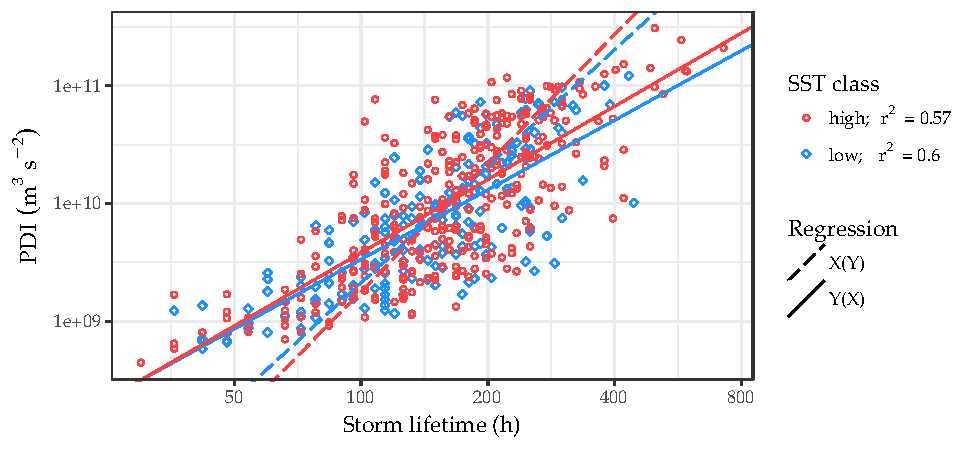
\includegraphics[width=\textwidth]{images/scatterplot-epac}
	\caption{Scatterplot of the joint distribution and regression analysis for the $PDI$ and lifetime of storms for the Northeast Pacific basin}
	\label{fig:epac-scatterplot}
\end{figure}

\begin{table}[H]
	\centering
	\begin{tabular}{cccccc}
		\toprule
		\toprule
		$X$ & $Y$ & SST class & $\hat{\beta}_{0}$ & $\hat{\beta}_{1}$ & $R^{2}$ \\
		\midrule
		\multirow{2}{*}{lifetime} & \multirow{2}{*}{$PDI$}
		 & Low  & \num{ 5.59 \pm 0.25} & \num{1.97 \pm 0.12} & \num{0.60} \\ % \pm 0.05} \\
		&& High & \num{ 5.45 \pm 0.23} & \num{2.07 \pm 0.10} & \num{0.57} \\ % \pm 0.04} \\
		\midrule
		\multirow{2}{*}{$PDI$} & \multirow{2}{*}{lifetime}
		 & Low  & \num{-0.83 \pm 0.18} & \num{0.30 \pm 0.02} & \num{0.60} \\ % \pm 0.05} \\
		&& High & \num{-0.55 \pm 0.14} & \num{0.28 \pm 0.01} & \num{0.57} \\ % \pm 0.04} \\
		\bottomrule
	\end{tabular}
	\caption{Linear regression coefficients obtained performing OLS on the Northeast Pacific basin data}
	\label{tab:epac-ols-coefs}
\end{table}

\begin{table}[H]
	\centering
	\begin{tabular}{cccccccc}
	\toprule
	\toprule
	$X$   & $Y$   & $T^{(1)}$ & $T^{(2)}$ & $T^{(3)}$ & $T^{(4)}$ & $T^{(5)}$ & $T^{(6)}$ \\
	\midrule
	lifetime & $PDI$ & $0.149$ & $0.103$ & $0.027$ & $0.437$ & $0.661$ & $1.099$ \\
	$PDI$ & lifetime & $0.285$ & $0.028$ & $0.027$ & $1.273$ & $1.254$ & $2.527$ \\
	\bottomrule
	\end{tabular}
	\caption{Value of the test statistics for Northeast Pacific basin data set using OLS}
	\label{tab:base-epac-ols-statistics}
\end{table}
